\chapter{Biological Background}
\label{ch:biological}

Drug design is a complex, costly, time-consuming process with a low average success rate of 2.1\%~\cite{hay_clinical_2014}. While companies usually require 10-15 years to develop a new drug, during which they often spend upwards of 12 billion dollars, the number of drugs approved by the United States' Food and Drug Administration (FDA) has been decreasing since 1995. The probability of a compound entering a phase I trial approved by the regulatory authority is less than 10\% and the ultimate number of compounds investigated that make it to market is approximately $1/30,000$. Further, as the need personalized medicine increases, so does the difficult to develop new drugs, and new strategies to develop drugs are necessary~\cite{hay_clinical_2014}~\cite{ashburn_drug_2004}.

Drug repositioning is the process of finding new uses outside the scope of the original medical indication for existing drugs~\cite{ashburn_drug_2004}.It is more efficient, less-costly, and less-risky than the conventional drug development (Figure ~\ref{fig:drug_repo_process}). It takes 1-2 years to find targets and 8 years to develop a repositioned drug with 1.6 billion dollars on average. The major advantage of drug-repurposing approaches is that, for an existing drug, both the preclinical information and the clinical profiles (pharmacokinetic, pharmacodynamic, and toxicity) are already available, thereby reducing the development risk. Accordingly, a drug compound can rapidly enter late-stage clinical trials, reducing development cost and time~\cite{novac_challenges_2013}.Figure 1 displays the comparison between \textit{de novo} drug development and drug repurposing processes.

Drug repositioning can be performed experimentally or computationally. The latter technique has been widely used to identify new indications for an existing drug (drug-centric) and for identifying effective drugs for treating a disease (disease-centric) by using a strategy of similarity assessment between drugs and/or diseases~\cite{park_review_2019}.

\begin{figure}[!h]
    \centering
    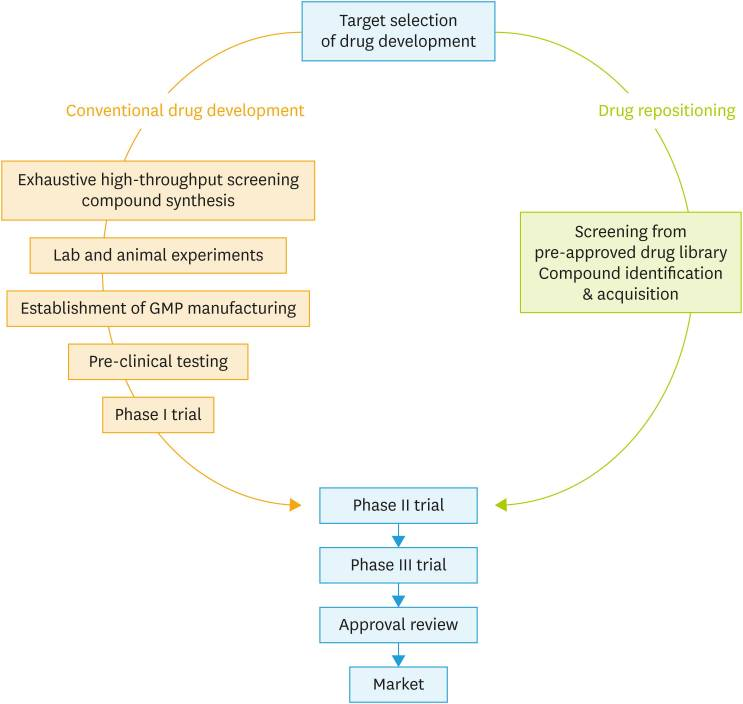
\includegraphics[scale=0.35]
    {figures/drug_repo_process.png}
    \captionsetup{justification=centering}
    \caption [A comparison of conventional drug development and drug repositioning]{\label{fig:drug_repo_process} A comparison of conventional drug development and drug repositioning. Figure adapted from~\cite{kobayashi_current_2019}}
\end{figure}

There are two trends of computational drug repositioning. While the first trend is to make use of high-throughput data including genomics, proteomics, chemoproteomic, and phenomics~\cite{park_review_2019}. which is flawed by noisy data and limitations of computational methods. For example, Zhang \textit{et al.} (2019) warned that when using genomics data, it is unreasonable to treat each single nucleotide polymorphism (SNP) equally when using the elastic net algorithm because of their different importance in epigenetic studies~\cite{dai_survey_2015}. The second trend is the development of repositioning algorithms based on retrospective analysis and database maintenance for experimental data, for which the challenge is to apply appropriate methods to integrate and exploit heterogeneous data.

Even computational drug repositioning has its limitations, but it’s still a promising method. Several examples of successful repurposed drugs exist in fields such as oncology, diabetes, leprosy, and inflammatory bowel disease. Alfedi \textit{et al.} (2019) performed a high‐throughput screening of a library containing 853 FDA approved drugs by using a cell‐based reporter assay to monitor variation of frataxin amount to accelerate the development of a new therapy for Friedreich's ataxia~\cite{kalathur_unihi_2014}.They found that \textit{etravirine} represented a promising candidate as a therapeutic for Friedreich's ataxia. Hassan \textit{et al.} (2019) designed a computational and enzyme inhibitory mechanistic approach to fetch promising drugs from the pool of FDA approved drugs against \ac{AD}. They found that \textit{cinitapride} can be used as a possible therapeutic agent in the treatment of \ac{AD}~\cite{law_drugbank_2014}. Besides the methods of these two examples, in recent years, network-based drug repositioning strategy is also widely used for predicting novel drug candidates of disease. 

\section{Network-based Drug Repositioning} \label{network_based}

Network-based drug repositioning has been recently widely used for finding new links between drugs and diseases. Biological networks $G = (V, E)$ consist of nodes $v \subset V$ that can be genes, proteins, anatomies, biological processes, compounds, diseases, etc., and their relationships (i.e., edges) $e \subset E$ . Network is a useful data structure from which algorithms can extract structure and semantic information for drug repositioning. Different types of network-based drug repositioning strategies are reviewed below based on the content of network ~\cite{lotfi_shahreza_review_2018}.

\subsection{Gene Regulatory Networks}

Molecular perturbations that occurred due to drug administration or a disease can be represented and exploited by building gene regulatory networks, and then the network can be used to prioritize nodes in existing networks to select candidate genes for drug repositioning.

Chen \textit{et al.} (2016)~\cite{chen_network_2016} made use of multiple information sources such as gene mutations, gene expression data, functional connectivity, and proximity of module genes based on mining a human functional linkage network for inversely correlated modules of drug and disease gene targets to identify candidates for treating breast and prostate cancer. Two subnetworks were extracted for each drug: one contained upregulated disease genes which were down regulated by the drug and the other one contained downregulated disease genes which were upregulated by the drug. The correlation relationship between the drug and the disease can be exploited from these two sub-networks. For case study, 5 FDA-approved drugs were identified as drug candidates that can serve as potential therapeutic treatments for breast cancer based on therapeutic index tests (e.g., toxic dose, dose for therapeutic response).

While this kind of method can be effective, the signature for a disease or a drug is not always clearly defined, and drug-target gene perturbations may not be detectable. Other network with more solid data needs to be generated and exploited for drug repositioning ~\cite{lotfi_shahreza_review_2018}.

\subsection{Protein-Protein Interaction Networks}

Protein-protein interaction \ac{PPI} networks are often used to identify similar proteins for drug targeted proteins based on the assumption that proteins targeted by similar drugs are functionally related and are ‘close’ in the PPI network~\cite{dai_survey_2015}. Some example PPI network data resources include UniHi~\cite{kalathur_unihi_2014}, DrugBank~\cite{law_drugbank_2014}, GeneCards~\cite{safran_genecards_2010}, Gene Expression Omnibus\ac{GEO}~\cite{clough_gene_2016}, Genotator~\cite{wall_genotator:_2010}, STRING~\cite{szklarczyk_string_2019}, the Kyoto Encyclopedia of Genes and Genomes\ac{KEGG}~\cite{kanehisa_kegg_2019}, Online Mendelian Inheritance in Man\ac{OMIM}~\cite{hamosh_online_2005}, and the iRef Index database~\cite{razick_irefindex:_2008}, Keane \textit{et al.} (2015)~\cite{keane_protein-protein_2015} represented mitochondrial dysfunction and autophagic dysregulation in the cellular MPP\footnote{+} model, a neuronal in vitro disease model containing dopaminergic neurons allow the testing of PD drug candidates~\cite{braungart_caenorhabditis_2004},for parkinson’s disease (PD) by generating a PPI networks for respective model. Next, for each node, they extracted topological features and calculated the betweenness centrality, a measure of the number of shortest paths across the network that include the node. The differences in betweenness centrality between each network were calculated to indicate the importance of the node in connecting autophagy and mitochondrial dysfunction in the MPP$^+$ system. The reseachers hypothesized that manipulating nodes with high change in betweenness centrality would regulate MPP$^+$ toxicity. At last, they prioritized P62, GABARAP, GBRL1, and GBRL2 as novel targets associated for PD.

The limitation of this method is that the PPI data has a high degree of variance and it is incomplete due to the diverse range of experimental sources. An integrated and detailed network is required to build a more informative PPI network by standardizing and filtering the PPI data.

\subsection{Drug-Target Interaction Networks}

Drug-target interaction\ac{DTI} networks represent the physical interactions of drugs with their targets as swell as their mechanisms of action (e.g., inhibition, agonism, antagonism, reverse agonism). Several data sources include DrugBank~\cite{law_drugbank_2014}, KEGG LIGAND, KEGG GENES, KEGG DRUG, KEGG BRITE~\cite{kanehisa_kegg_2019}, Drug Combination Database\ac{DCDB}~\cite{liu_dcdb_2014}, Matador~\cite{gunther_supertarget_2008}, BRENDA~\cite{schomburg_brenda_2002}, SuperTarget~\cite{gunther_supertarget_2008}, MalaCards online system~\cite{rappaport_malacards:_2017}, and \ac{STITCH}~\cite{kuhn_stitch:_2008}.

Yamanishi \textit{et al.}~\cite{yamanishi_prediction_2008} used DTI networks to demonstrate that if two drugs have similar structure, they have a higher chance to interact with similar target proteins. Likewise, two target proteins with high sequence similarity are more likely to interact with similar drugs. Yan \textit{et al.} (2016)~\cite{yan_prediction_2016} built a heterogeneous network G consisting of drugs and their targets, a drug-drug network \textit{U} and a target-target network \textit{V} extracted from \textit{G} based on similarities between drugs and targets respectively. Between the two sub-networks, drugs and targets were connected with edges E to form a bipartite network G = (U, V, E). They developed and applied a method, LPMIHN, to the network to rank targets if the query is a drug and vice versa.

The main limitation of this method is that few drug-target data sets are available. The prediction of models is highly dependent on the training data, so such models cannot predict drugs without target information. Another limitation is that negative samples are difficult to find since there is a scarcity of experiments that were conducted for verifying negative drug-target samples~\cite{chen_semi-supervised_2013}. The solution for the first problem is to make use of highly similar drugs to predict targets (or highly similar targets to predict drugs ) for those without relevant information~\cite{alaimo_recommendation_2016}. In machine learning scenarios, the second problem can be addressed with positive-unlabeled learning, in which negative samples can be sampled randomly from unlabeled drug-target pairs. However, this does not address the overarching issue the biocuration community has with structuring negative knowledge. Positive unlabeled learning is discussed in more detail in the methods section.

\subsection{Drug Similarity Networks}

Drug similarity networks support inference methods that rely on the assumption that drugs with similar structures have similar biological effects. The similarities of drugs can be measured by using two-dimensional topological fingerprints, 3D conformations, or biological effects (side effects or gene expression patterns).

Drug similarities are usually measured by structure similarities with fingerprints~\cite{willett_similarity-based_2006} or chemical graph, which is based on the assumption that compounds with similar structures have similar activity. But this method suffers from that drugs similar in structures often have very different biological effects~\cite{stumpfe_exploring_2012}. To compensate for such a limitation,\ac{SITAR}~\cite{perlman_combining_2011} used 5 similarity measurements for drug-drug pairs, which are chemical similarities, side effect similarities~\cite{kuhn_stitch:_2008}, gene expression profiles similarities, and \ac{ATC} classification. However, this method is still flawed by the similarity measuring and lack of structure information of compounds. 

\subsection{Disease-Disease Networks}

Disease-disease networks consist of disease nodes and disease-disease similarity edges. They can be generated from resources like DrugBank~\cite{law_drugbank_2014}, \ac{OMIM}~\cite{hamosh_online_2005}, and \ac{DO} ~\cite{schriml_disease_2012}. This network strategy is to find novel drug-disease relationship by measuring the similarity between diseases based on the assumption that similar diseases are similar to be treated by similar drugs. How to measure the similarity between diseases is critical to this disease-disease network strategy. Van Driel \textit{et al.} (2006)~\cite{van_driel_text-mining_2006} created MimMiner to calculate disease similarity based on phenotypes. Huimin Luo \textit{et al.} (2016)~\cite{luo_drug_2016} improved MimMiner by exploiting the correlative relationships between diseases by comparing the existence of their common drugs. They provided a case study where Levodopa is predicted to treat \ac{AD}, which had already been tested in clinical trial~\cite{noauthor_clinicaltrials.gov_nodate}.

\subsection{Disease-Side effects Networks}

Many drugs induce some unintended effects on the living organisms in addition to the desired effects by interacting with off-targets~\cite{wu_network-based_2013}~\cite{yang_finding_2008}. Those side effects provide a human phenotypic profile for the drug, which suggest additional disease indications. The rationale for drug repositioning based on side effect profiles is that side effects and indications are both measurable behavioral or physiological changes in response to treatment, and if drugs treating a disease share the same side effect, there might be some underlying mechanism-of-action \ac{MoA} linking this disease and the side effects. The side effect may thus serve as a phenotypic “biomarker” for this disease.

Yang \textit{et al.} (2011) hypothesized that if a given drug is associated with common side effects as drugs that treat a given disease, then it should also be a candidate for treating that disease. They generated a network with diseases, drugs and side effects. Disease-drug associations were extracted from PharmGKB~\cite{thorn_pharmgkb:_2013} and drug-side effect associations are extracted from the \ac{SIDER}~\cite{kuhn_sider_2016}. A quantitative structure-activity relationship model was built to compensate for the absence of side effect profiles for many drugs. Then they built naive Bayes models to predict indications for 145 diseases using the side effects as features. The \ac{AUC-ROC} was above 0.8 in 92\% of these models, which indicated that closer attention should be paid to the side effects observed in trials not just to evaluate the harmful effects, but also to rationally explore the repositioning potential based on this “clinical phenotypic assay”. Also, they provided a case study that porphyria was suggested to act as antidiabetics and delusions might help with depression~\cite{yang_systematic_2011}.

Not many drug repositioning methods are based on this strategy due to some limitations. The relationships between phenotypes and \ac{MoA}s are unclear because outcomes of drugs' MoAs are highly dependent on the organism’s genetic map, medication history, and other traits. Therefore, similar phenotypes are not always caused by similar targets. Even the assumption is valid, many drugs don't have comprehensive and accurate side effects profiles. ~\cite{dai_survey_2015}~\cite{wu_network-based_2013}~\cite{lotfi_shahreza_review_2018}.

\subsection{Integrated Networks}

Networks discussed in previous sections usually contain only two or three types of nodes, such as drugs, targets, diseases, gene signatures, etc. If an integrative network including drugs, targets, phenotypes, diseases, and pathways, can be built to represent the \ac{MoA} (Figure \ref{fig:drug_thrapy_model}) of a drug, the predictions would be more accurate based on rich information in the network.

\begin{figure}[!h]
    \centering
    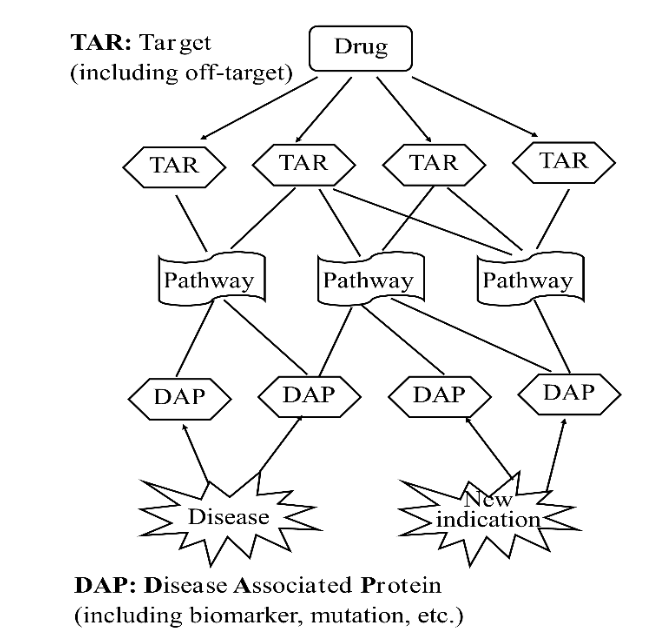
\includegraphics[scale=0.35]
    {figures/drug_therapy_model.png}
    \captionsetup{justification=centering}
    \caption[Drug Therapy Model]{\label{fig:drug_thrapy_model} Drug Therapy Model. Figure adapted from~\cite{ye_drug_2016}}
\end{figure}

Luo \textit{et al.} (2017)~\cite{luo_network_2017} built a pipeline, DTINet, which applied learned features to drug-target prediction for drug repositioning. Random Walk with Restart\ac{RWR} and Diffusion Component Analysis\ac{DCA} were used to generate learned features. DTINet focused on learning a low-dimensional vector representation of features, which accurately illustrated the topological properties of individual nodes in the heterogeneous network, and then made prediction based on these representations via a vector space projection scheme. They predicted novel interactions between three drugs and cyclooxygenase proteins and demonstrated potential applications of these identified cyclooxygenase inhibitors as a role of preventing inflammatory diseases.

There are four types of nodes and six types of relationships in DTINet. They extracted the drug nodes from the DrugBank database (Version 3.0)~\cite{knox_drugbank_2011} and the protein nodes from the Human Protein Reference Database (HPRD) (Release 9) ~\cite{keshava_prasad_human_2009}. The disease nodes were obtained from the Comparative Toxicogenomics Database ~\cite{davis_comparative_2013}. The side-effect nodes were collected from the SIDER database (Version 2)~\cite{kuhn_side_2010}. They imported the known DTIs as well as drug–drug interactions from DrugBank (Version 3.0)~\cite{knox_drugbank_2011}. The protein–protein interactions were downloaded from the HPRD database (Release 9) ~\cite{keshava_prasad_human_2009}. The drug–disease and protein–disease associations were extracted from the Comparative Toxicogenomics Database~\cite{davis_comparative_2013}. They also included the drug–side-effect associations from the SIDER database (Version 2)~\cite{kuhn_side_2010}.

Integrative networks contain more comprehensive information for \ac{MoA} but the limitation is that only a few network representation learning methods are designed for heterogeneous network. Also, it is more difficult to build a high quality network with diverse sources and the standard of adding an edge between two nodes needs to be normalized, for example, the threshold of similarity between nodes and the standard of differentially expressed genes in an anatomy.

\section{Methods used in Computational Drug Repositioning}

Recently, repositioned drugs account for 30\% of newly marketed drugs in the US~\cite{plenge_validating_2013}. In the meantime, the explosive and large-scale growth of molecular, genomic and phenotypic data of pharmacological compounds is enabling the development of new area of drug repurposing called computational drug repurposing. There are three main categories, machine learning methods, network-based methods and text-mining methods ~\cite{park_review_2019}.

\subsection{Machine Learning Methods}

Machine learning techniques that have been applied for drug repositioning include logistic regression,\ac{SVM}, random forest, neural networks, and deep learning~\cite{park_review_2019}. In this thesis, binary classification is applied to distinguish drug-disease pairs, so only logistic regression and\ac{SVM} are discussed here.

Logistic regression is a widely used statistic model. It is often applied for binary classification problem, in which samples are usually labeled as two classes, positive and negative. Logistic regression is used to describe data and to explain the relationship between one dependent binary variable and one or more nominal, ordinal, interval or ratio-level independent variables and predict labels with given input.

In biological science, Ayers \textit{et al.} applied penalized regression methods to select pertinent predictors for a phenotype~\cite{ayers_snp_2010}. Himmelstein \textit{et al.}~\cite{himmelstein_systematic_2017} used logistic regression for predicting new drug-disease link in Hetionet. Muslu \textit{et al.} trained a logistic regression model by learned features of disease-targets pairs from GAT2VEC to predict targets of a disease~\cite{alaimo_recommendation_2016}. Liu \textit{et al.}~\cite{liu_similarity-based_2015} generated a web service SPACE (Similarity-based Predictor of ATC CodE), which for each submitted compound, will give candidate ATC codes which is ranked according to the decreasing probability\_score. Behind this web service, is a logistic regression model trained by drug similarity features including chemical structures, target proteins, gene expression, side-effects and chemical–chemical associations.

\ac{SVM} is another popular binary classification model. The objective of the \ac{SVM} is to find a hyperplane in an N-dimensional space (N is the number of features) that distinctly partition the data points into two parts by maximizing the margin from both sides to the hyperplane.Napolitano \textit{et al.}~\cite{napolitano_drug_2013} combined molecular target, drug chemical structure, and gene expression similarity into one feature matrix. Then they predicted drug therapeutic class by an \ac{SVM} approach based on feature matrices. Shameer \textit{et al.} (2018)~\cite{shameer_prioritizing_2018} use RepurposeDB~\cite{shameer_systematic_2018} and DrugBank~\cite{wishart_drugbank_2018} as datasets and ChemVec as feature engineering strategy to train supervised classification algorithms (naïve Bayes, random forest, \ac{SVM}s, and an ensemble model combining the three algorithms).

In this thesis, the elastic net, a penalized logistic regression, is used to predict new drug-disease edges because the logistic regression gives not only class predictions but also probability predictions, which is used for ranking the drug candidates in drug repositioning.

\subsection{Network-based Methods}

Based on the graph topological properties, the entities in the same cluster are similar to each other. For biological network, proteins, genes, drugs should cluster with similar nodes. This approach is used to identity drug-disease, drug-target relationships~\cite{xue_review_2018}. Lu \textit{et al.} used chemical-chemical interactions and chemical-protein interactions to select candidate compounds that had close associations with approved lung cancer drugs and lung cancer-related genes. K-means clustering and a permutation test were applied to remove compounds with low possibilities to treat lung cancer. The final results suggest that the remaining compounds in cluster has structural similarities with approved drugs for lung cancer and they have potential anti-lung cancer activities~\cite{lu_identification_2016}.

The workflow of network-based propagation approach is that prior information of source nodes propagate to other nodes in network. This approach contains two types: local approaches and global approaches. Local approaches take limited information into account~\cite{xue_review_2018}. Global approaches are more accurate by exploring more information. Martinez \textit{et al.} created DrugNet, a new methodology for drug-disease and disease-drug prioritization by integrating drugs, proteins, and diseases into network. They rank the nodes in these networks according to their distance to a query set of nodes. DrugNet achieved a mean AUC-ROC value of 0.9552 ± 0.0015 in 5-fold cross validation tests, which suggests DrugNet could be very useful for discovering new drug use~\cite{martinez_drugnet:_2015}.

\subsection{Semantic and Texting-Mining}

The structured information in databases is only a fraction of all knowledge, the biomedical and pharmaceutical literature contains a huge amount of  unstructured information available for drugs and diseases, from which new indications of existing drugs can be found through text-mining method. Su \textit{et al.} (2017)~\cite{su_systematic_2017} used the text mining tools I2E (Linguamatics) and PolyAnalyst (Megaputer) to extract \ac{SAE} data from randomized trials in ClinicalTrials.gov. Through a statistical algorithm, a PolyAnalyst workflow ranked the drugs where the treatment arm had fewer predefined \ac{SAE}s than the control arm, indicating that potentially the drug is reducing the level of \ac{SAE}. The results indicated that \textit{telmisartan} may be viable as a repurposed prevention for colon cancer and this was reported by few researches that Telmisartan exerted anti-tumor effects by activating peroxisome proliferator-activated receptor-$\gamma$~\cite{li_telmisartan_2014}~\cite{pu_telmisartan_2016}~\cite{wu_increase_2016}.

Ngo \textit{et al.} (2017) made use of continuous-bag-of-words model from word2vec~\cite{mikolov_efficient_2013} to get word embeddings for cancer related drugs and diseases~\cite{ngo_application_2016}. The raw corpus is a subset of PubMed abstracts downloaded in October 2013, filtered by the keyword “cancer”. After getting embeddings from word2vec model, they performed hierarchical clustering for testing the quality of word embeddings and \ac{SVM} classification to learn and predict possible relations between drugs and diseases. The clustering showed anti-cancer drugs condensed in one cluster which indicated that the word embedding catched the characteristic of words and the \ac{SVM} classification model achieved 87.6\% accuracy of drug-disease relations in cancer treatment. Also the model succeeded in discovering novel drug-disease relations that were actually reported in recent studies. For example, repositioning of Clarithromycin to anticancer agent was reported in 2015~\cite{pantziarka_repurposing_2015}. Based on the fact that the corpus were downloaded in 2013, the prediction was valid and indicated that the classification of concatenated word vector was a promising approach to in-silico screening of drug-disease relations for drug repositioning.

\subsection{Validation of Computational Drug Repositioning}

The evaluation of computational drug repositioning is usually case studies or unbiased validation methods such as \ac{AUC-ROC}, which summarise the trade-off between the true positive rate and false positive rate for a predictive model using different probability thresholds, \ac{AU-PR}, which summarise the trade-off between the true positive rate and the positive predictive value for a predictive model using different probability thresholds. Some researchers experimentally validated their results with \textit{in vivo} experiments. The flaw of case studies is that finding evidences in other research paper is inefficient and difficult. Another method, unbiased validation method, is also flawed by the assumption that all drug-disease indications not in databases (e.g., DrugCentral) are false. To address these concerns, Adam \textit{et al.}~\cite{shameer_systematic_2018} present repoDB, a database of approved and failed drugs and their indications. repoDB approved indications were drawn from DrugCentral, which contains United Medical Language System \ac{UMLS} indications mapped from free-text mentions in drug labels. In this thesis, due to the purpose of comparing this work to previous work, the case studies, \ac{AUC-ROC} and \ac{AU-PR} are used for validating. Applying repoDB will be one of the future work.

\section{Rephetio Approach}

All the networks discussed above in the section \ref{network_based} contain at most 4 types of nodes and 6 types of relationships. But the \ac{MoA} (Figure 2) behind drug-disease relationships are very complicated and involve many other entities such as anatomy, pathways, molecular functions, etc., so an integrative network is necessary to represent comprehensive biological knowledge accumulated from previous studies. For methods of computational drug repositioning, machine learning methods are very powerful to classify and predict relationships between entities, but one must for machine learning is that feature vectors are indispensable.

Himmelstein \textit{et al.} (2017) ~\cite{himmelstein_systematic_2017} generated a heterogeneous network, Hetionet, including biological knowledge from 29 different databases, which contains 11 types of nodes and 24 types of edges, in order to fulfill the absence of a comparatively comprehensive network in network-based drug repositioning field. Furthermore, they generated engineered feature (e.g., DWPC) vectors and the engineered features representing prevalence of metapaths were interpreted by extracting weights of features from logistic regression model. After prediction of novel drug-disease indication, 10 most supportive paths in the network could be found by their algorithm, which not only gives a decent explanation for predictions but also inspiring clues for scientists to verify the predicted indications.

\subsection{Hetionet}

Nodes consist of 1552 small molecules and 137 complex diseases, also genes, anatomies, pathways, biological processes, molecular functions, cellular components, perturbations, pharmacologic classes, drug side effects, and disease symptoms.

Gene nodes are from Entrez Gene, which belongs to the National Center for Biotechnology Information ~\ac{NCBI} database for gene-specific information. Entrez Gene maintains records from genomes that have been completely sequenced, assigns unique, stable and tracked integers as identifiers to each gene sequence. The content of Entrez Gene is integrated and curated in an automatic way through NCBI's Reference Sequence project~\cite{maglott_entrez_2011}.

Entrez Gene was chosen but not \ac{HGNC} identifier due to few advantages of Entrez Gene compared to \ac{HGNC}. Entrez Gene is more specific to humans, geneIDs are less prone than ambiguous gene symbols in ~\ac{HGNC}, and integration of Entrez Gene with many other NCBI services such as HomoloGene can relate orthologous genes across species~\cite{himmelstein_entrez_2015}.

Disease nodes are from \ac{DO}~\cite{schriml_disease_2012}, which is a database provides standard hierarchical disease terms. However, the method of Rephetio requires distinct and non-redundant nodes, which means that no terms should be an ancestor or descendant of any other term. Therefore, disease terms should be chosen from an appropriate level, specific enough to be clinically relevant and general enough to be well annotated. To create this DO slim, 108 diseases from GWAS catalog in hetio and 63 cancer terms from TOPNodes\_DOcancerslim are combined. Then some overlapped diseases are removed. At last, 137 disease terms are selected for Hetionet.

Compound nodes are from DrugBank with drugs approved, small molecules containing InChI structures~\cite{law_drugbank_2014}. Interacting proteins (targets, enzymes, transporters, carriers) for each drug are extracted for Hetionet. There are two criterias for proteins to be included. One is that the interaction is between a drug and single protein. A target which is a "protein group" (e.g., GABA-A receptor (anion channel) and NMDA receptor) is excluded. Also, a target which is not a protein but a DNA or phosphate is excluded too. Another one is that The protein should be mapped to an entrez gene. At last, 19,906 interactions for 5,878 drugs and 3,757 genes are extracted~\cite{himmelstein_protein_2015}. The connectivity fingerprints are calculated with Morgan/circular [63] method in order to get the similarities between compounds. RDkit module was used to calculate similarities of compounds with Dice Coefficient (Equation 1, a is the number of “1” in fingerprint of A, b is the number of “1” in fingerprint of B, c is the intersection of fingerprints of A and B) [64]. The similarity threshold is 0.5. Then Compounds from DrugBank are mapped to 30 other compound resources using UniChem. The mapping is based on atomic connectivity and ignores differences in small molecular details, but the mapping with PubChem is based on exact InChi string matches.

\begin{equation}
S(A,B) = 2 *c / a +b
\end{equation}

Anatomy nodes are from \ac{UBERON}~\cite{mungall_uberon_2012}, to represent anatomical structures. \ac{UBERON} integrates cross-species ontology consisting of over 6,500 classes representing a variety of anatomical entities, organized according to traditional anatomical classification criteria.

Symptom nodes are from ~\ac{MeSH}, a controlled vocabulary produced by the \ac{NLM} for cataloging biomedical information, used to annotate PubMed and MEDLINE. Two record types are processed in Hetionet: Descriptors and Supplementary Concept Records ~\cite{himmelstein_user-friendly_2016}~\cite{himmelstein_mining_2015}.

Pathway nodes are from WikiPathways, Reactome, and the \ac{PID}~\cite{schaefer_pid:_2009}. Only protein-coding human genes (as Entrez Gene IDs) are included ~\cite{himmelstein_dhimmel/pathways_2016}~\cite{pinero_disgenet:_2015}. Pathways files are downloaded as TSV (Tab Separated Values) file and overlapped pathways are removed. At last, 1,862 human pathways (1,341 from Reactome, 298 from WikiPathways, and 223 from PID) are generated.

Disease-gene edges are from DisGeNET. Disease node is from Disease Ontology, and the gene is represented as Entrez Gene. DisGeNET integrates data from expert curated repositories, \ac{GWAS} catalogues, animal models and the scientific literature, and the data are homogeneously annotated with controlled vocabularies and community-driven ontologies ~\cite{pinero_disgenet:_2015}.

Diseases-differentially expressed genes edges are from STARGEO, which aims to provide disease-specific expression signatures on a broad scale with crowdsources \ac{GEO} annotation and performs case-control analyses based on user queries. In summary, STARGEO defines case-control queries for 66 diseases. Of these diseases, 49 contained sufficient data which means multiple studies with at least 3 samples per class. Hetionet used STARGEO's random effects meta-analysis and applied a false discovery rate (FDR) p-value threshold of 0.05 to identify differentially expressed genes for each disease. 48,688 Disease–downregulates–Gene and 50,287 Disease–upregulates–Gene relationships were identified ~\cite{himmelstein_stargeo_2015}.

Disease-symptom occurrence edges, disease-disease occurrence edges, disease-localization edges and anatomy-disease co-occurrence edges are calculated between \ac{MeSH} terms. 23 million journal articles are provided in the \ac{NLM}. Skilled subject analysts at the \ac{NLM} typically assign 10–12 \ac{MeSH} terms per article and denote a subset of these terms as major topics. They infer relationships between nodes in Hetionet based on MEDLINE co-occurrence ~\cite{himmelstein_mining_2015}.

Gene-anatomy differential expression edges are from Bgee~\cite{bairoch_bgee:_2008}, a database that integrates gene expression data from both microarray and RNA-seq experiments. The Bgee curators annotate samples by their species, anatomical structure, and developmental stage. Bgee leverages anatomical and developmental ontologies to call whether a gene is present or absent and under/over-expressed in a given condition. Gene expression profiles for human anatomical structures (tissues) are generated from Bgee for Hetionet, including whether a gene is expressed in an anatomy, whether a gene is overexpressed or underexpressed in an anatomy.

Protein-protein interaction edges are from three sources, Human Interactome Database (HID) ~\cite{luck_reference_2019}, Incomplete Interactome ~\cite{menche_uncovering_2015}, hetio-dag ~\cite{himmelstein_heterogeneous_2015}. The edge exists when two proteins physically interact. Besides, for combining an orthogonal resource to the protein interactions, \ac{ERC} between genes ~\cite{himmelstein_systematic_2017}, which assesses whether two genes have a similar evolutionary history are calculated. An edge is added when \ac{ERC} of two genes are bigger than 0.75.

Drug-disease edges are from PharmacotherapyDB ~\cite{himmelstein_announcing_2016}, an open catalog of medical indications between small molecule compounds and complex human diseases. Containing two parts, Disease Modifying and Symptomatic, both are reviewed by multiple physicians. Diseases and drugs are coded with Disease Ontology and DrugBank identifiers for integrative analysis. Four resources are integrated, LabledIn ~\cite{khare_labeledin:_2014}, MEDI-HPS~\cite{wei_development_2013} , EHRLink~\cite{mccoy_development_2012}, PREDICT~\cite{gottlieb_predict:_2011}. Disease modifying is defined as "a drug that therapeutically changes the underlying or downstream biology of the disease" and Symptomatic as "a drug that treats a significant symptom of the disease." When one of them is satisfied, one edge between the drug and the disease is built.

Compound-gene edges are from \ac{LINCS}~\cite{koleti_data_2018}. A database provides perturbational profiles across multiple cell and perturbation types, as well as read-outs, at a massive scale. One compound in Hetionet could be matched to multiple \ac{LINCS} compounds. A single consensus transcriptional profile across multiple signatures is calculated to reduce redundancy~\cite{himmelstein_computing_2015}.

Drug-side effects edges are from SIDER 4~\cite{kuhn_sider_2016}, a project to combine data on drugs, targets and side effects into a more complete picture of the therapeutic mechanism of actions of drugs and the ways in which they cause adverse reactions. It contains data on 1430 drugs, 5,880 \ac{ADR}s and 140,064 drug-\ac{ADR} pairs, which is an increase of 40\% compared to the previous version. For more precise analyses, they extracted the frequency with which side effects occur for 39\% of drug-\ac{ADR} pairs, and 19\% of those pairs can be compared to the frequency under placebo treatment. \ac{SIDER} furthermore contains a data set of drug indications, extracted from the package inserts using Natural Language Processing. These drug indications are used to reduce the rate of false positives by identifying medical terms that do not correspond to \ac{ADR}s.There are some other nodes and edges are contained in Hetionet, as shown in Table \ref{tab:nodes_edges_hetio}

\begin{table}[!ht]
    \centering
    \begin{tabular}{|p{3cm}|p{5cm}|p{7cm}|}
        \hline
        \textbf{Nodes$\backslash$ Edges} & \textbf{Source} & \textbf{Annotation} \\
        \hline
        Pharmacologic class & DrugBank ~\cite{law_drugbank_2014} & It gives the information that which pharmacologic class one drug is belonged to. \\
        \hline
        Gene Ontology &Gene Ontology & Entrez GeneIDs related to GO terms are provided and set as symbols \\
        \hline
        Pathway-protein edges & WikiPathways ~\cite{kutmon_wikipathways:_2016}, Reactome ~\cite{croft_reactome:_2011}, and Pathway Interaction Database (PID) ~\cite{schaefer_pid:_2009} & As discussed in the section pathway node\\
        \hline
        Pharmacologic class-drugs edges & Drug Central & If the drug is belonged to a certain pharmacologic class, an edge is created between them. \\
        \hline
        GO terms-Entrez Gene edges & Gene Ontology ~\cite{the_gene_ontology_consortium_gene_2015} and Entrez Gene ~\cite{maglott_entrez_2011} & If the gene is related to the GO term, an edge is added between them. \\
        \hline
        Compound-target edges & DrugBank ~\cite{law_drugbank_2014} & As discussed in the section compounds nodes \\
        \hline
        Chemical-chemical similarity edges & DrugBank ~\cite{law_drugbank_2014} & 
The similarity is calculated with finger prints and the threshold is 0.5. More information is in the section compound nodes. \\
        \hline
    \end{tabular}
    \captionsetup{justification=centering}
    \caption{Short introduction for some nodes and edges in Hetionet}
    \label{tab:nodes_edges_hetio}
\end{table}

\subsection{Rephetio Methods}

Himmelstein \textit{et al.} adapted an algorithm originally developed for social network analysis and applied it to Hetionet to identify patterns of efficacy and predict new uses for drugs. The algorithm performs edge prediction through a machine learning framework that accommodates the breadth and depth of information contained in Hetionet ~\cite{himmelstein_heterogeneous_2015}.

\subsubsection{Engineered Features}

For capturing the connections between compound nodes and disease nodes, Himmelstein \textit{et al.} ~\cite{himmelstein_systematic_2017} engineered topological features to train logistic regression model for drug repositioning. The \ac{DWPC}, prior probability, and node degrees for 14 meta-edges are included in features.

\ac{DWPC} represents the prevalence of a specific metapath. In Figure \ref{fig:DWPC}, on the left is a hypothetical graph, the source node is IRF1, the target node is Multiple Sclerosis. There are several paths from IRF1 to Multiple Sclerosis, one kind of path is one metapath like ‘G-e-T-l-D’. Only one path fits this kind of metapath, which is IRF1-expression-Leukocyte-localization-Multiple-Sclerosis. In this path, node IRF1, connecting with two nodes (node type is ‘Target’) with edge type of ‘expression’, has a metaedge-specific degree of 2. Then get all metaedge-specific degrees of one path to count \ac{PDP}. If there are more than one paths of the same metapath type, add 0\ac{PDP} of all paths together to get \ac{DWPC}.

\begin{figure}[!h]
    \centering
    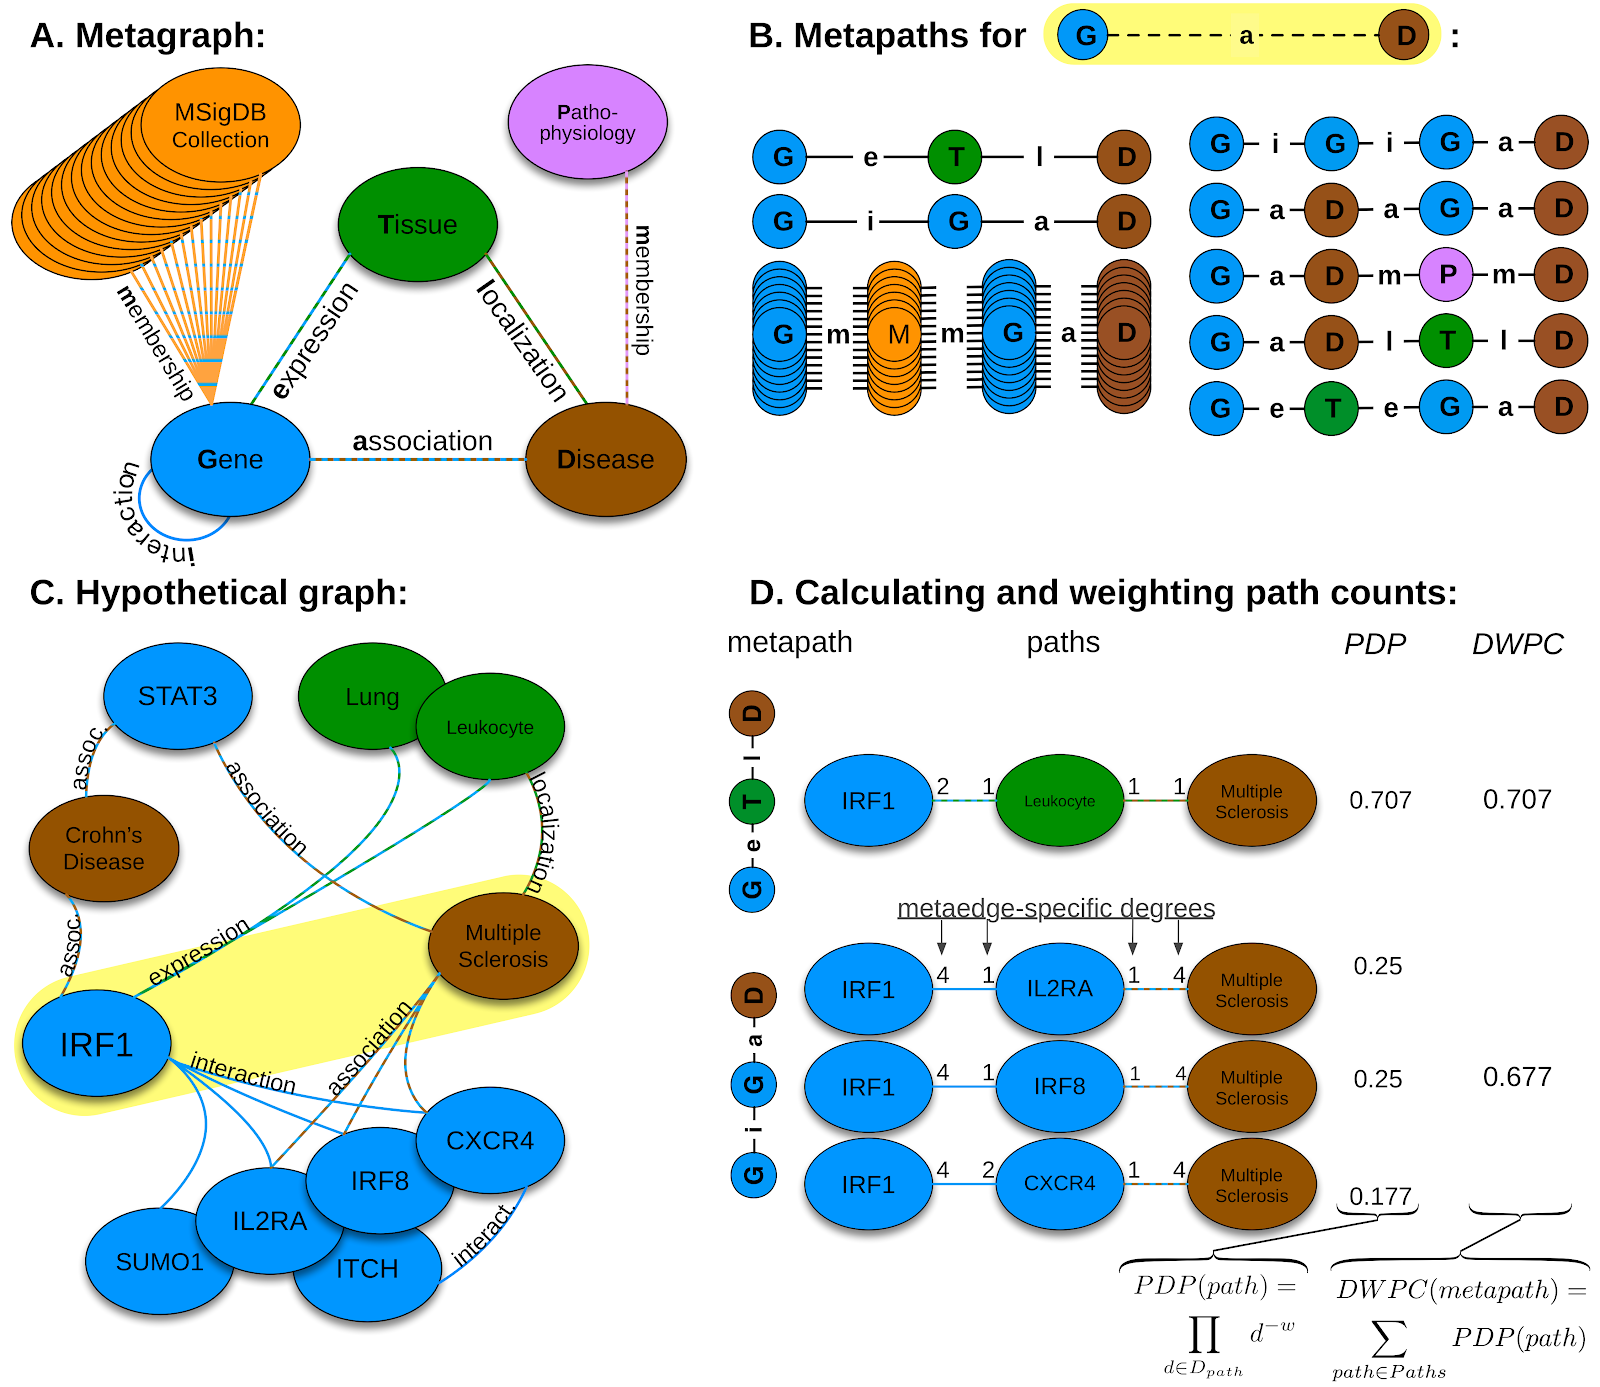
\includegraphics[scale=0.2]
    {figures/DWPC.png}
    \captionsetup{justification=centering}
    \caption[DWPC calculation workflow]{\label{fig:DWPC} DWPC calculation workflow. Figure adapted from~\cite{himmelstein_systematic_2017}}
\end{figure}

They evaluated all 1206 metapaths that traverse from compound to disease and have a length of 2–4 with \ac{DWPC}, and compared the performance of each metapath to a baseline computed from permuted networks. The permutation preserved node degree while eliminating edge specificity, in order to isolate the portion of un-permuted metapath performance resulting from actual network paths. They refer to the permutation-adjusted performance measure for a metapath as $\Delta$\ac{AUC-ROC}. A positive $\Delta$\ac{AUC-ROC} indicates that paths belonging to the type of metapath tended to occur more frequently between treatments than non-treatments, after accounting for different levels of connectivity (node degrees) in the network. In general terms, $\Delta$\ac{AUC-ROC} assesses whether paths of a given type were informative of drug efficacy [46]. The \ac{DWPC}\ac{DWPC} features were chosen based on the evaluation of $\Delta$\ac{AUC-ROC} and other standards. At last, 142 \ac{DWPC} features left for representing drug-disease pairs~\cite{himmelstein_hetnet_2016}.

ince Himmelstein \textit{et al.} engineered features and chose features manually, after prediction, it is possible to interpret the result according to coefficient of each feature. They extracted metapaths of which the coefficient given by the logistic regression model were positive based on the assumption that metapath features (e.g., \ac{DWPC}) with positive coefficients and positive logistic regression term are considered to contribute positively. Then they find the most supportive paths according to the metrics of \ac{DWPC}.

Figure \ref{fig:most_supportive_hetio} shows the ten most supportive paths for treating nicotine dependence with bupropion. These supportive paths possibly explain why bupropion could be used to treat nicotine dependence.

\begin{figure}[!h]
    \centering
    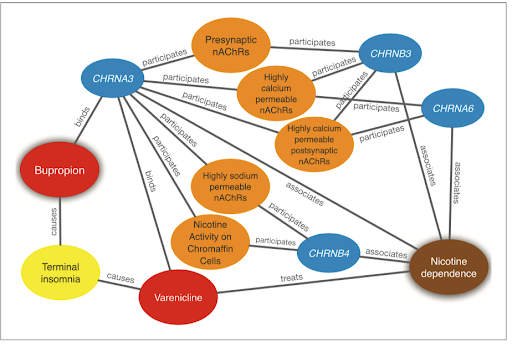
\includegraphics[scale=0.5]
    {figures/10_most_supportive.png}
    \captionsetup{justification=centering}
    \caption[Evidence supporting the repurposing of bupropion for smoking cessation]{\label{fig:most_supportive_hetio} Evidence supporting the repurposing of bupropion for smoking cessation. Figure adapted from \cite{himmelstein_systematic_2017}}
\end{figure}

\subsection{Shortcomings of Rephetio Method and Learned Features}

Usually scientists engineered features from similarities based on structures or phenotypes~\cite{perlman_combining_2011}, but in network-based drug repositioning, engineering feature vectors becomes more difficult because of a lack of powerful algorithm to represent biological entities especially in heterogeneous network. Furthermore, engineering features such as \ac{DWPC} can only represent limited characteristic of the network. While \ac{DWPC} for one metapath represents the prevalence of this type of metapath, many other topological information such as neighbours and vicinity are missed. Also, engineered features are are not generalizable. If drug-target features are wanted, \ac{DWPC}s have to be evaluated and chosen again, which makes this methodology less extensible.

With the advancement of network representation learning methods, it is possible to generate feature vectors with other methods (e.g., node2vec). Muslu \textit{et al.} (2019)~\cite{muslu_guiltytargets:_2019} used a genome-wide protein-protein interaction network annotated with disease-specific differential gene expression to predict targets for drugs with logistic regression model trained by learned features from DeepWalk model. They evaluated the approach on six diseases of different types (cancer, metabolic, neurodegenerative) within a 10 times repeated 5-fold stratified cross-validation and achieved AUC-ROC values between 0.92-0.94, significantly outperforming a previous approach from Emig \textit{et al.} ~\cite{emig_drug_2013}, which relies on manually engineered topological features.

Luo \textit{et al.} (2017)~\cite{luo_network_2017} applied another method, \ac{DCA}, ~\cite{cho_diffusion_2015} to generate learned features for predicting novel drug-target associations in DTINet. \ac{DCA} is a method to capture the inherent topological features of a network and represent it as low-dimension feature vectors, which uses diffusion methods for network to get the distribution of nodes with restart random walk. Then approximate each of these distributions by constructing a multinomial logistic model, parameterized by low-dimensional feature vector(s), for each node. Feature vectors of all nodes are jointly learned by minimizing the Kullback-Leibler (KL) divergence (relative entropy) between the diffusion and parameterized-multinomial logistic distributions. Also, their results outperformed the state-of-art methods for drug-target predictions, which indicated that DTINet with learned features can provide a practically useful tool for integrating heterogeneous information to predict new drug–target interactions and repurpose existing drugs.

The shortcomings of engineered features can be overcomed by learned features, which is easier to be generated and keep comparatively comprehensive topological and semantic features of the network. \ac{DCA} and DeepWalk are both random walk based methods, but the way of them to catch the co-occurrence properties of nodes are different. \ac{DCA} simply makes use of multinomial logistic model to catch the co-occurrence probabilities between nodes calculated before training, but DeepWalk uses neural network to keep not only the co-occurrence probabilities but also how nodes pairs co-occur with each other by feeding node pairs to the neural network. Furthermore, Ngo \textit{et al.} ~\cite{wu_increase_2016} applied language model (continuous bag-of-word, similar to skip-gram) for drug repositioning as a successful try. Based on these studies, random-walk and language model based network representation learning methods (e.g., node2vec) are promising to represent topological features of a heterogeneous network and for further drug repositioning task. The Computational Background section discusses the methods used in this thesis.